\chapter{Research question}

In this bachelor thesis research will be conducted on how functional reactive programming can be beneficial to development of real-time web applications. The research question that will be answered is the following: "Can functional reactive programming be used to make developing real-time web applications more efficient?".

\section{Metrics}
\label{sec:metrics}

The metrics that will be used to assess whether the use of FRP is beneficial to real-time web application development are the following: Amount of code, readability, learning curve, performance and extensibility.

\section{Approach}

The first part of this bachelor thesis will research FRP and real-time dataflow on the web today. Because this bachelor thesis is applied to the web all code examples will be in JavaScript.

To come to a conclusion a practical case study will be conducted. The research question will be evaluated by implementing a simple case in a traditional imperative style and in a declarative FRP style. The metrics defined in section \ref{sec:metrics} will then be used to compare the two implementations and formulate a conclusion.

The case that will be implemented in this bachelor thesis will be a simple text-based chat application. This is the simplest example of a real-time application with full-duplex communication. To measure extensibility a feature will be added to the finished application and the degree of difficulty will be assessed.

\chapter{Real-time on the web} % (fold)
\label{sec:realtime}

\section{HTTP Polling} % (fold)
\label{sub:polling}

The simplest way to do real-time on the web is to poll a server via Ajax at a certain interval. This is a simple but very primitive way to update data in real-time. This technique has multiple downsides. Firstly the communication is not really real-time and your data will always be out of date because of the usage of an interval. Secondly this technique also increases load on your server because it has to handle a lot of requests from the clients. This makes scaling with a HTTP polling architecture very cumbersome \cite{poll-socket}. Lastly this technique cannot do two-way communication between server and client so this it is not suitable for real-time communication \cite{poll-socket}.

\section{HTTP long polling} % (fold)
\label{sub:long-polling}

HTTP long polling is a variation on HTTP polling. The client will still poll the server for new data but the server will keep the request open until it has new data. After the client gets a response it will immediately send a new request, repeating the process \cite{long-poll} (see figure~\ref{figure:long-poll}). This technique resolves most downsides of classic HTTP polling but it still cannot facilitate two-way communication between server and client \cite{poll-socket}.

\begin{figure}[H]
	\centering
	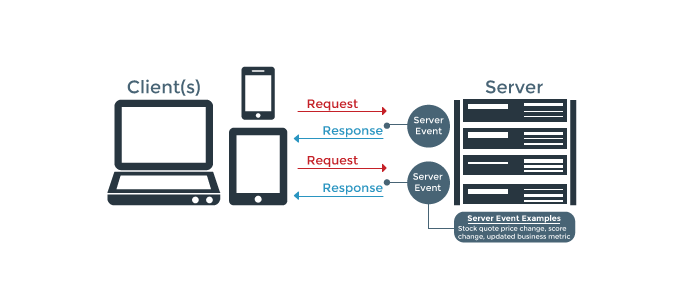
\includegraphics[width=1\textwidth]{long-poll}
	\caption{Long polling \cite{long-poll}}
	\label{figure:long-poll}
\end{figure}

\section{WebSockets} % (fold)
\label{sub:websockets}

HTML5 WebSockets are a full-duplex communication channel (see figure~\ref{figure:socket}) that operates through a single socket over the web. HTML5 WebSockets is not just another small improvement over conventional HTTP communications \cite{poll-socket}, it is a completely new communication protocol. Under the hood WebSockets are built on TCP; they do not use HTTP except for establishing the connection \cite{socket-wiki}. Browser support for WebSockets is excellent, all major browsers support them \cite{socket-browser}.


\begin{figure}[H]
	\centering
	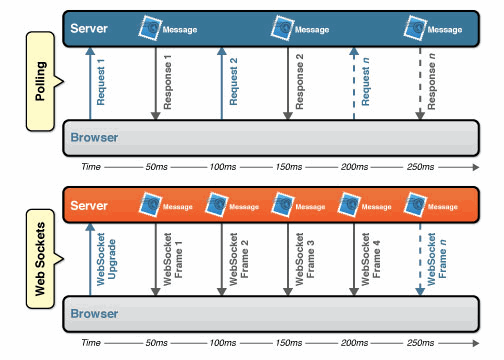
\includegraphics[width=0.8\textwidth]{socket}
	\caption{Comparison of HTTP polling and WebSockets \cite{poll-socket}}
	\label{figure:socket}
\end{figure}

\subsection{Libraries} % (fold)
\label{sub:websockets-implementations}

There are many libraries that abstract away some of the complexity from the WebSocket protocol. The most popular WebSocket libraries at the time of writing are Socket.IO, Primus, ws and Faye. The most popular reasons to choose a library over using the vanilla version are elegant fallbacks for browsers that do not support WebSockets and automatic reconnection.

\section{WebRTC} % (fold)
\label{sub:webrtc}

WebRTC is full-duplex communication protocol developed and open sourced by Google in 2010 \cite{webrtc-intro}. After that WebRTC was standardised by the IETF and the W3C \cite{webrtc-intro}. Now there are implemented open standards for real-time, plugin-free video, audio and data communication. WebRTC allows real-time peer-to-peer communication of audio, video and arbitrary data between browsers. A server is only needed to set up the initial connection between peers, this process is called signaling \cite{webrtc} (see figure~\ref{figure:signal}).

\begin{figure}[H]
	\centering
	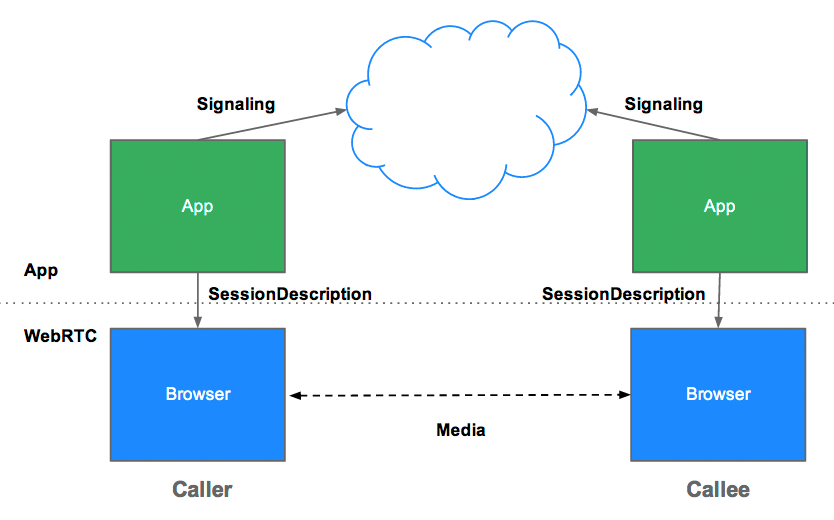
\includegraphics[width=0.8\textwidth]{signal}
	\caption{Signaling process for WebRTC \cite{webrtc-intro}}
	\label{figure:signal}
\end{figure}

WebRTC's P2P connection model further increases scalability and simplicity of real-time applications \cite{webrtc}. However WebRTC also has some caveats. Even though it has been around for 4 years now browser support is still lacking at the time of writing \cite{webrtc-browser}. It is also hard to implement WebRTC in a client-server architecture \cite{hn} as it was primarily made for P2P communication.

\chapter{Functional reactive programming} % (fold)
\label{sub:frp}

FRP is a programming paradigm that integrates the idea of asynchronous dataflows into functional programming. This provides an elegant way to express computation for areas that involve a lot of time related variables such as animation and user interface rendering \cite{frp-wiki}\cite{frp-haskell}. 

\section{Functional programming} % (fold)
\label{sub:fp}

Functional programming is a programming paradigm that models computation as a composition of pure functions without mutating any state \cite{func-js}. It is a declarative programming paradigm. One of the biggest advantages of functional programming is that by using pure functions it becomes much easier to reason about the behavior of a program \cite{func-js}.

Functional programming has its origins in lambda calculus, a system in mathematical logic for expressing computation based on operations and variables \cite{lambda}.

\subsection{Declarative programming}

In declarative programming a program describes what to do, rather than how to do it. This is the opposite of classic imperative programming \cite{intro-func}. The difference between the two is best explained by example. Listing~\ref{listing:imp} and listing~\ref{listing:dec} both show an implementation of a function called \code{double}. The function takes an array and returns another array with all elements doubled. Listing~\ref{listing:imp} shows an imperative implementation of this function, the function explicitly says to loop over the elements, double them and add them to an empty array. Listing~\ref{listing:dec} shows a declarative implementation of this function, it only says what we want to happen to the elements in the array.

\begin{lstlisting}[caption=Imperative implementation of the double function,label=listing:imp]
function double (arr) {
	let results = [];
	for (let i = 0; i < arr.length; i++) {
		results.push(arr[i] * 2);
	}
	return results;
}
\end{lstlisting}

\begin{lstlisting}[caption=Declarative implementation of the double function,label=listing:dec]
function double (arr) {
	return arr.map(item => item * 2);
}
\end{lstlisting}


\subsection{First-class functions}

In functional programming functions are first-class citizens. This means that functions can be treated like any other value. They can be created, stored in data structures and passed into or returned from other functions.

\subsubsection{Pure functions}

Pure functions have two defining characteristics. The first is that the function's result only depends on its arguments, given the same arguments the function will always return the same value \cite{intro-func}. The second characteristic is that pure functions do not cause any side effects such as mutations to data structures or output to I/O devices \cite{intro-func}.

\subsubsection{Higher order functions} % (fold)
\label{sub:fp-order}

Higher order functions are functions that either take a function as an argument, return a function or both. This is a simple concept that makes function composition possible. Function composition helps keeping functional programs readable and easy to reason about \cite{intro-func}.

An example of a higher order function in JavaScript is the \code{map} function of the Array prototype (see listing~\ref{listing:dec}). This function takes a function as an argument. The invokeTwice function in listing~\ref{listing:ho} is an example of a higher-order function that returns a function.

\begin{lstlisting}[caption=Higher order function composition,label=listing:ho]
const invokeTwice = f => subject => f(f(subject));
const double = x => x * 2;
const quad = invokeTwice(double);

quad(10); // 40
invokeTwice(double)(10); // 40
\end{lstlisting}

The \code{invokeTwice} function will take a function as an argument and return a function that applies the first function twice on its argument. The example also shows how \code{invokeTwice} can be composed together with other functions such as \code{double}. A function like \code{invokeTwice} that takes one argument at a time and returns a function taking the next argument is called a curried function. \cite{func-js}.

\subsection{Immutability}

Functional programming promotes the use of immutable data structures, most functional languages even enforce it \cite{func-js}. Immutability means that a data structure cannot be changed. If an operation is done on an immutable object it copies the value, mutates it and returns it as a new object. This helps eliminate bugs where an object enters a state that was not predicted by the programmer \cite{intro-func}.

\subsection{Other functional jargon}

There are many other terms associated with functional programming but these are out of scope for this thesis. This chapter only serves to give a basic understanding of the functional programming paradigm.

\section{Reactive programming}
\label{sub:rp}

Reactive programming is a programming paradigm that deals with asynchronous data streams \cite{intro-reactive}. These data streams will then propagate their changes to other parts of the application; this is the observer pattern \cite{observer}. Reactive programming has three main objects: an observable or a stream, an observer or subscriber and a scheduler \cite{intro-reactive}.

An observable will emit values over time. An observable can be infinite or it can complete after a certain number of emitted values. Observers can subscribe to these streams and get notified whenever the observable emits a value, throws an error or completes (see listing~\ref{listing:observer} for an example). Schedulers decide on which thread an observer's code should run and when.

\begin{lstlisting}[caption=An observable and observer in RxJS,label=listing:observer]
const someObservable$ = Observable.from([1,2,3]);

someObservable$
	.subscribe(
		value => console.log(value),
		error => console.err(error),
		completed => console.log('completed')
	);
	
// output: 1, 2, 3, completed
\end{lstlisting}

\subsection{Operators}

Typically a FRP library or language includes a lot of operators \cite{intro-reactive} so that observables can be easily manipulated. In FRP operators are pure functions that take an observable and return another observable. A simple example of an operator is the delay operator. This operator is available in RxJS and returns the input observable with every value delayed by a specified amount of time \cite{delay} (see figure~\ref{figure:delay}). Because operators return a new observable, operators can be easily chained after one another.

\begin{figure}[H]
	\centering
	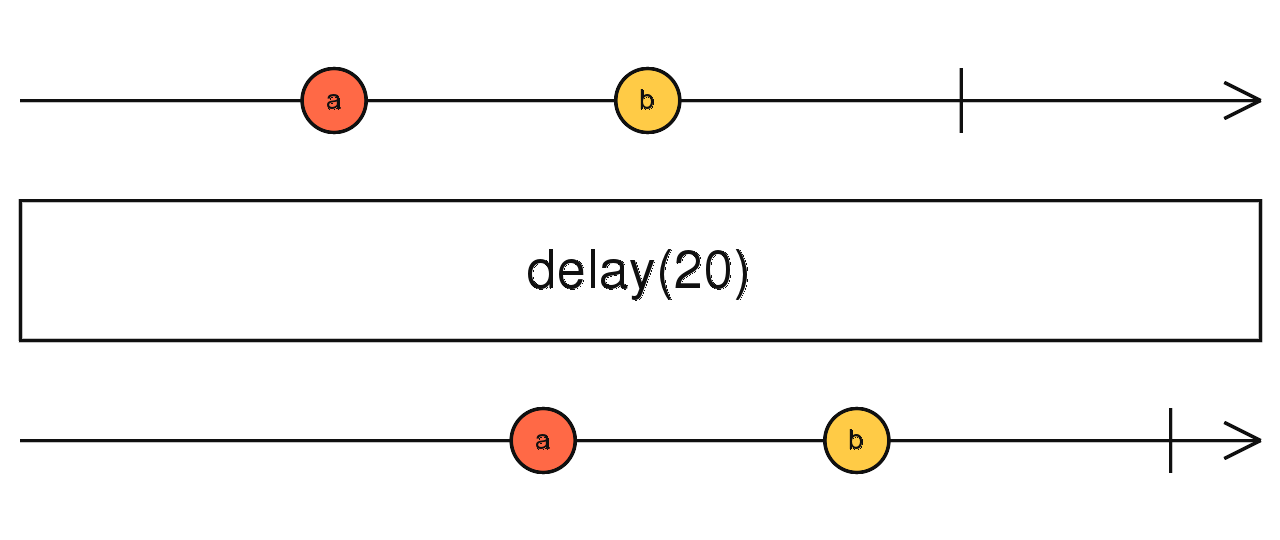
\includegraphics[width=\textwidth]{delay}
	\caption{The delay operator in RxJS: marble diagram \cite{delay}}
	\label{figure:delay}
\end{figure}

An example of operators on a data stream can be seen in figure~\ref{figure:stream}, this example illustrates a stream of clicks by a user. The events in the stream are first grouped by throttling them for 250ms. Afterwards they are mapped to the length of the groups and finally they are filtered so that only groups of clicks equal or larger than 2 remain. This example shows really well how reactive programming helps with handling asynchronism and concurrency in modern applications.

\begin{figure}[H]
	\centering
	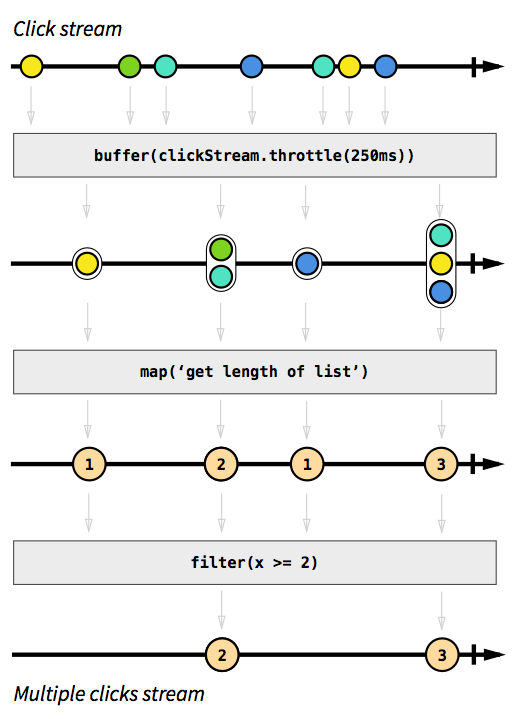
\includegraphics[width=0.7\textwidth]{stream}
	\caption{Stream of clicks \cite{intro-reactive}}
	\label{figure:stream}
\end{figure}

\subsection{Visualizing observables}

The biggest roadblock in adoption of reactive programming by developers has been the steep learning curve. Reactive programming forces the developer to think about dataflow in a different way. In reactive programming data arrives over time and is immutable. Essential in learning to think reactive is being able to visualize how observables work over time.

Marble diagrams are the main tool that is used today to visualize observables. These diagrams can be great tools to not only understand the core concepts of reactive programming but also understand the functionality of individual operators (see figure~\ref{figure:delay} and \ref{figure:stream}).

\subsection{Debugging}

The main area where reactive programming falls short today is debugging. Since operators tend to be one line arrow functions it is not possible to set a breakpoint inside them. This results in a lot of developers either using console statements or having to convert operator functions to functions with a body every time they want to debug. Moreover stack traces tend to be longer and less useful than those from imperative programming. Because everything is asynchronous and a lot of work is done internally in the FRP library, stack traces tend to show only the errors internal to the library which is not useful for the developer \cite{debug}. An important sidenote is that Paul Irish announced new features coming to Chrome Devtools during Google I/O 2017 that will allow developers to debug asynchronous code more efficiently \cite{devtools}. Stack traces will become more descriptive and developers will be able to step inside one line arrow functions such as \code{Promise.then()} \cite{devtools}.

RxJS 5 is a complete rewrite of RxJS 4 and one of it's biggest improvements is its shorter stack traces making it easier for developers to debug their code \cite{debug}. Other tools one can use to debug and reason about reactive code are marble diagrams and dependency graphs \cite{debug}. Marble diagrams let developers visualize observables and find mistakes in their reasoning. Dependency graphs will help the developer understand what observables your current observable depends on and for what. This helps identify problems where an observable the current observable depends on is not behaving the way the developer expects it to. An example of a dependency graph is shown in figure~\ref{figure:depgraph}.

\begin{figure}[H]
	\centering
	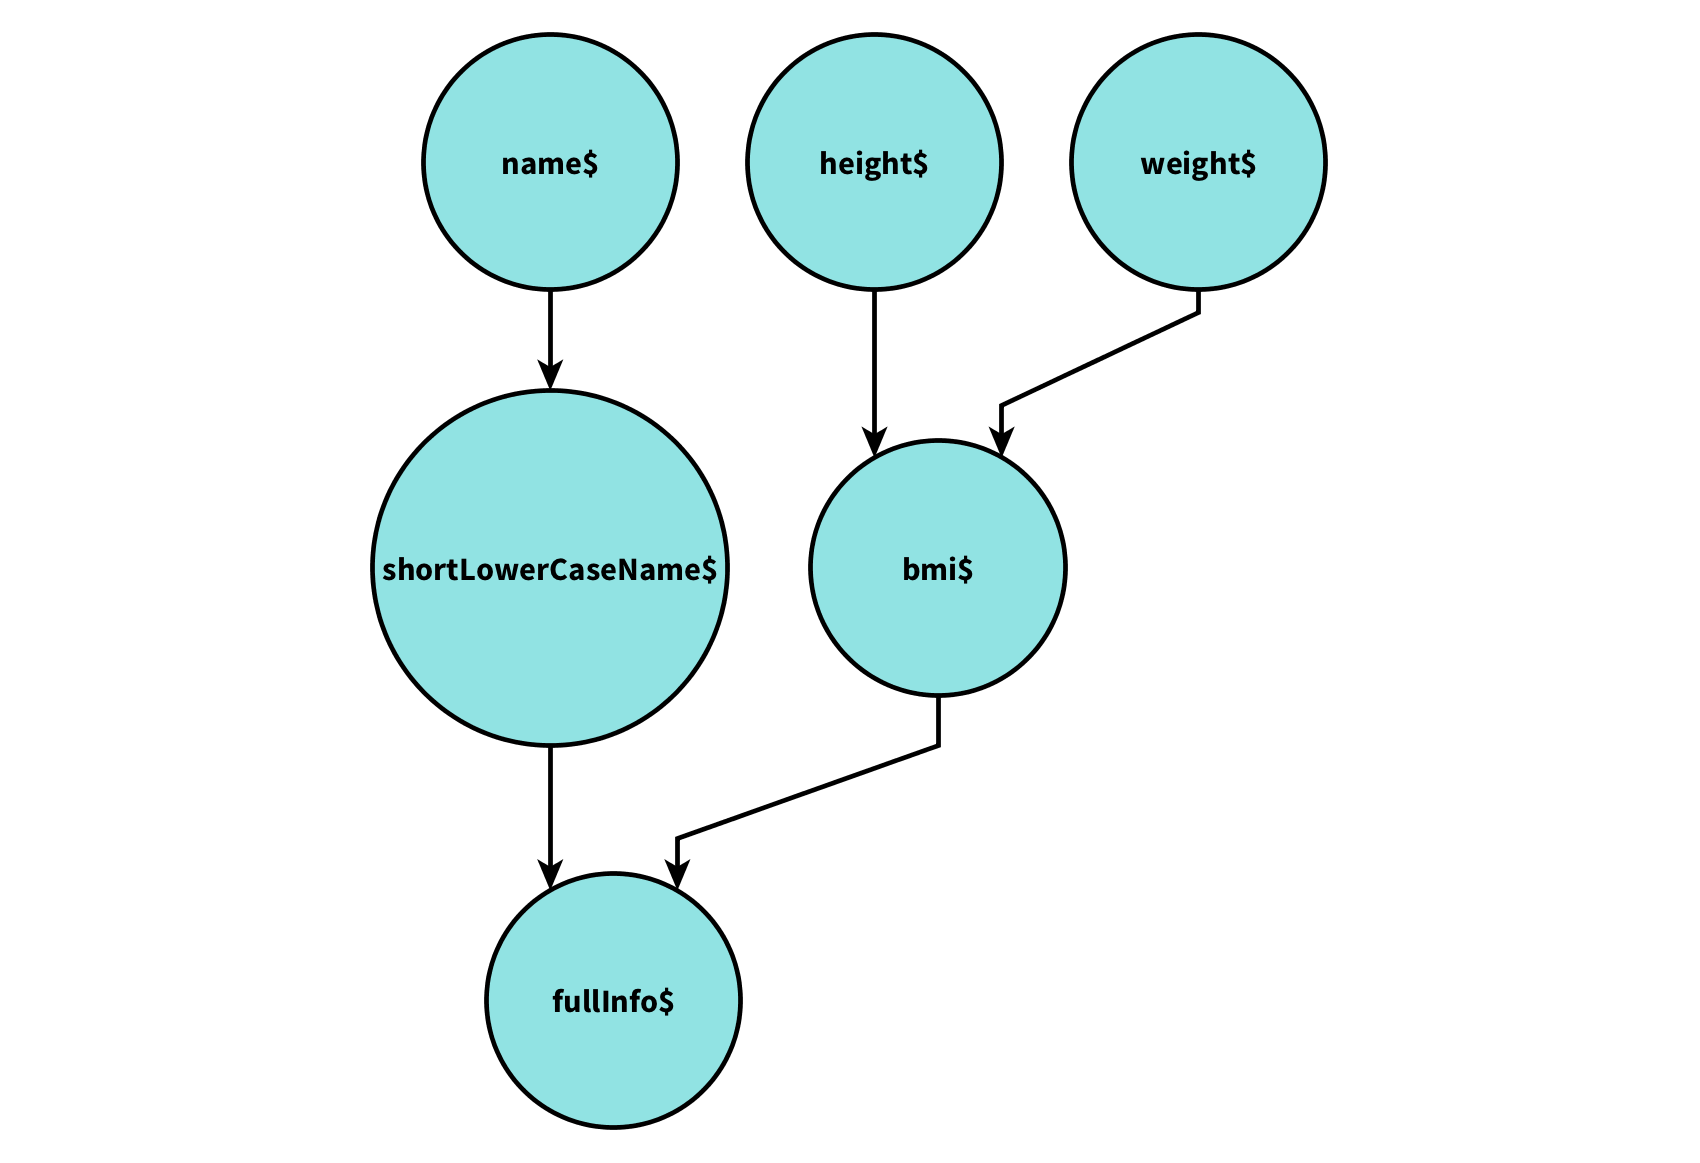
\includegraphics[width=0.9\textwidth]{dep}
	\caption{A dependency graph of observables in a BMI calculator \cite{debug}}
	\label{figure:depgraph}
\end{figure}

The figure above shows the dependency graph of a simple Body Mass Index (BMI) calculator. The code associated with this example can be seen in listing~\ref{listing:bmi}. The code example assumes that the input streams \code{name\$}, \code{weigth\$} and \code{height\$} are already instantiated before this code runs. 

\begin{lstlisting}[caption=Reactive BMI calculator source code \cite{debug},label=listing:bmi]
const shortLowerCaseName$ = name$
	.map(name => name.toLowerCase())
	.filter(name => name.length < 5);

const bmi$ = weight$
	.combineLatest(
		height$,
		(weight, height) => Math.round(weight / (height * height * 0.0001))
	);

const fullInfo$ = shortLowerCaseName$.combineLatest(bmi$);
\end{lstlisting}

\subsection{Hot and cold observables}

Observables can be either hot or cold. The way the producer is linked with the observable defines whether it is hot or cold. A producer is an object that provides values to an observable. The producer can be an iterator, an event of a DOM element, a WebSocket etc. The pseudocode in listing~\ref{listing:hot} shows how a producer is linked up to an observable for hot and cold observables.

\begin{lstlisting}[caption=Hot and cold observables in RxJS \cite{hot},label=listing:hot]
// Cold observable
const cold = new Observable((observer) => {
	const producer = new Producer();
	// have observer listen to producer here
});

// Hot observable
const producer = new Producer();
const hot = new Observable((observer) => {
	// have observer listen to producer here
});
\end{lstlisting}

When creating a cold observable a producer is made for each observer. This means that if there is no observer subscribed there is also no producer being instantiated. This is the reason why observables in RxJS need to be subscribed to in order to emit anything at all. Cold observables are unicast \cite{hot}. This means that every producer will only emit its data to one observer. As a result this can cause issues when working with very rapidly changing data such as time. Because every observer has its own producer, the time at which observers receive the same data can differ \cite{hot}.

For a hot observable the producer is set up even if no observer is subscribed to it. When multiple observers subscribe to the same observable the producer will be shared. Emitted data from the producer will be multicast to all observers \cite{hot}. In most FRP libraries including RxJS observables are cold by default. Observables in RxJS can be made hot with the publish and share operators \cite{hot}, subjects (see section~\ref{subjects}) are always hot.

\subsection{Subjects} \label{subjects}

Subjects are an additional data structure provided in some FRP libraries. Subjects behave exactly like observables but their data does not come from a producer. Instead data can be pushed manually to the subject \cite{subjects}. This helps bridge the gap between imperative programming and reactive programming. Subjects make it easy for a programmer to integrate stateful data into an observable. Since subjects are compatible with all observable operators they can be combined with other observables. It is considered to be a bad practice though and whenever it can be avoided it is advised to use observables over subjects \cite{subjects}.

\section{FRP in JavaScript}

Because of JavaScript's unopinionated nature, choice of programming paradigm is left to the developer. JavaScript also has a lot of the ingredients needed for FRP built into the language. Functions in JavaScript are already first-class citizens of the language \cite{func-js}. Arrow functions allow JavaScript functions to be reasoned about as lambda calculus and finally ES2015 introduced a few functional array functions such as map, reduce and filter \cite{es2015}.

Because of these characteristics JavaScript is an excellent language for functional reactive programming.

\subsection{Asynchronous Javascript}

Dealing with asynchronism has always been one of the biggest challenges of programming for the web. Over the years developers have employed different techniques to handle asynchronous code in JavaScript.

\subsubsection{Callbacks}

Callbacks are the simplest way to handle asynchronism in JavaScript. The principle is simple; a callback function is passed as an argument with another function. That function will then call the callback function when it finishes its work.

The problem with callbacks is that they quickly become unreadable when the programmer needs to compose different asynchronous actions. Listing~\ref{listing:cb} is an example of 3 asynchronous functions running one after the other. This example code is already pretty complex even though is accomplishes a very simple task.

\begin{lstlisting}[caption=Fetching data  with nested callbacks,label=listing:cb,float]
getData(function (err, x) {
	if(err) {
		console.error(`Oh no! an error: ${err}`);
		return;
	}
	getMoreData(x, function (err, y) {
		if(err) {
			console.error(`Oh no! an error: ${err}`);
			return;
		}
		other(x, y, function (err, z) {
			if(err) {
				console.error(`Oh no! an error: ${err}`);
				return;
			}
			...
		});
	});
});
\end{lstlisting}

\subsubsection{Promises}

Promises are an alternative way to handle asynchronous code. Promises were standardized in ES2015 but have been around for years in various libraries such as Bluebird \cite{promise}. The Promise API allows the developer to compose asynchronous code in a more declarative manner. A promise can either resolve and deliver a value or reject and throw an error.

Listing~\ref{listing:promise} shows the example of listing~\ref{listing:cb} rewritten with the JavaScript Promise API. The \code{Promise.catch()} function will handle all errors on a chain of promises.

\begin{lstlisting}[caption=Fetching data with the Promise API,label=listing:promise]
getDataPromise
	.then(x => getMoreDataPromise(x))
	.then(y => otherPromise(y))
	.then(z => ...)
	.catch(err => {
		console.error(`Oh no! an error: ${err}`);
	});
\end{lstlisting}

If the promises in the example would not depend on the result of the previous one the \code{Promise.all()} function could be used. This function will complete when all promises have resolved. The \code{Promise.all()} function will throw an error if one of the promises rejects \cite{prom-all}.

\subsubsection{Async/await}

Async functions and the async/await syntax was recently introduced to JavaScript in ES2017 \cite{async-await}. It is a new language construct to handle asynchronous code. The await operator will block code execution until an async function has completed. The example used in listing~\ref{listing:cb} and listing~\ref{listing:promise} is rewritten below in listing~\ref{listing:await} using the async/await syntax. 

\begin{lstlisting}[caption=Fetching data with the async/await keywords,label=listing:await]
async function getAllData() {
	try {
		const x = await getData();
		const y = await getMoreData(x);
		const z = await other(y);
		...
	} catch(err) {
		console.error(`Oh no! an error: ${err}`);
	}
}	
\end{lstlisting}

\subsubsection{Functional Reactive Programming}

FRP provides a more versatile API to handle asynchronous code than Promises and async/await. As Akash Agrawal correctly notes in his article "What Promises Do That Observables Can’t" observables completely overshadow promises in terms of functionality \cite{observables-promises}.

Listing~\ref{listing:observable-getdata} shows the example from the listings in the previous paragraphs rewritten using RxJS observables. The \code{getMoreDataObservable} and \code{getOtherObservable} function in this example return an observable based on their parameter. While the implementations with promises and async/await are slightly more concise FRP offers a lot more functionality than both. RxJS observables for example provide operators to cancel, buffer and debounce asynchronous code \cite{rxjs-ben}. Promises or async/await provide no API for those functionalities.

\begin{lstlisting}[caption=Fetching data with FRP (RxJS),label=listing:observable-getdata]
dataObservable$
	.flatMap(x => getMoreDataObservable(x))
	.flatMap(y => getOtherObservable(x))
	.catch(err => {
		console.error(`Oh no! an error: ${err}`);
	})
	.subscribe(z => {
		...
	});
\end{lstlisting}

\subsection{Current state}

Many libraries already bring FRP to JavaScript. The most popular ones at the time of writing are RxJS, xstream and Bacon.js \cite{intro-reactive}. There is also a proposal out there to bake an observable data structure into a future version of ECMAScript \cite{tc39}.

In 2013 Evan Czaplicki and Stephen Chong published a thesis at the Harvard University about the creation of Elm \cite{elm}. Elm is a practical FRP language with two important features: high-level abstractions to support simple, declarative FRP and purely functional graphical layout calculation \cite{elm}. Elm is also known for its excellent tooling and the absence of runtime errors in the language. Most importantly the Elm language is built on top of JavaScript and is made with the web in mind.

The FRP paradigm has been around for a very long time but it is still very new to the web platform. The need for a good abstraction to handle asynchronous code can be a driving factor to increase adoption of FRP in JavaScript. Possible support for observables in the JavaScript language can also further increase developer adoption in the future.


